\documentclass[12pt]{article}

\usepackage{float}

\usepackage{standalone}

\usepackage[utf8x]{inputenc}

%%% PAGE DIMENSIONS
\usepackage{geometry}
\geometry{a4paper}
\geometry{margin=2.54cm} % for example, change the margins to 2 inches all round

\usepackage{graphicx} % support the \includegraphics command and options

\usepackage[parfill]{parskip} % Activate to begin paragraphs with an empty line rather than an indent

%%% PACKAGES
\usepackage{booktabs} % for much better looking tables
\usepackage{array} % for better arrays (eg matrices) in maths
\usepackage{paralist} % very flexible & customisable lists (eg. enumerate/itemize, etc.)
\usepackage{verbatim} % adds environment for commenting out blocks of text & for better verbatim
\usepackage{subfig} % make it possible to include more than one captioned figure/table in a single float
% These packages are all incorporated in the memoir class to one degree or another...

\usepackage{multicol}
\usepackage{multirow}
\usepackage{xcolor}
\usepackage{amsmath}

\usepackage[T1]{fontenc}
\usepackage{lmodern}

\usepackage{makecell}

\renewcommand{\arraystretch}{1.1}

%%% HEADERS & FOOTERS
\usepackage{fancyhdr} % This should be set AFTER setting up the page geometry
\pagestyle{fancy} % options: empty , plain , fancy
\fancyhead[L]{\leftmark}
\fancyhead[C]{}
\fancyhead[R]{\rightmark}
\fancyfoot[L]{}
\fancyfoot[C]{}
\fancyfoot[R]{\thepage}
\renewcommand{\headrulewidth}{0pt}
\renewcommand{\footrulewidth}{0pt}

\fancypagestyle{plain}{
	\fancyhf{} % clear all header and footer fields
	\fancyfoot[R]{\thepage} % except the center
	\renewcommand{\headrulewidth}{0pt}
	\renewcommand{\footrulewidth}{0pt}
}

%%% BIBILIOGRAPHY
\usepackage[numbers]{natbib}
\bibliographystyle{vancouver}

%%% SECTION TITLE APPEARANCE
\usepackage{sectsty}
\allsectionsfont{\sffamily\mdseries\upshape} % (See the fntguide.pdf for font help)
% (This matches ConTeXt defaults)

%%% ToC (table of contents) APPEARANCE
\usepackage[nottoc,notlof,notlot]{tocbibind} % Put the bibliography in the ToC
\usepackage[titles,subfigure]{tocloft} % Alter the style of the Table of Contents
\renewcommand{\cftsecfont}{\rmfamily\mdseries\upshape}
\renewcommand{\cftsecpagefont}{\rmfamily\mdseries\upshape} % No bold!

\usepackage[bookmarks,bookmarksnumbered,bookmarksopen,hidelinks]{hyperref}

\usepackage{bookmark}


%%% TITLE
\title{Models for antibody data}
\author{Arseniy Khvorov, David Price, Annette Fox, Sheena G. Sullivan}
\begin{document}

%%% Title
\maketitle

%%% Main Contents

%\pagebreak
%==============================================================================
\section{Ha Nam application}

%------------------------------------------------------------------------------
\subsection{Scaled logit fit}

The scaled logit model was fit in a Bayesian way to better handle missing data and censored titre measurements. The full specification is

\begin{align*}
\begin{gathered}
Y_i \sim \text{Bernoulli}(p_i) \\
p_i = \frac{\lambda}{1 + \text{exp}(\beta_0 + \beta_T T_i)} \\
T_i \sim N(\mu, \sigma^2) \ \text{truncated}(L_{i}, H_{i}) \\
\mu \sim N(2, 2^2) \quad \sigma \sim \text{Exponential}(\text{rate} = 0.1) \\
\lambda \sim \text{Uniform}(0, 1) \\
\beta_0 \sim N(-15, 10^2) \quad \beta_T \sim N(5, 5^2)
\end{gathered}
\end{align*}

Where $i$ is observation index, $Y_i$ is infection status (0 --- infected (both symptomatic and asymptomatic), 1 --- not infected), $T_i$ is true log HI titre, $L_i$ is the low bound of observed HI interval (e.g. for observation of 20 this is log(20)), $H_i$ is the high bound of observed HI interval (e.g. for observation of 20 this is log(40)).

The prior distributions for the mean and standard deviation of log HI titres were chosen to be broad but still somewhat reflect the expected distribution in the general population --- mean high enough to allow a fair proportion (>20\%) to have titres above detectable level (log(10)) and standard deviation low enough to not result in titres above highest detectable level (log(1280)) to be more prevalent than titres between log(640) and log(1280).

The prior distribution for the baseline risk parameter $\lambda$ gives equal probability to all of its possible values. The prior distributions for the logistic curve parameters $\beta_0$ and $\beta_T$ was chosen to be spread around all of their plausible values --- $\beta_0$ is likely below 0 (otherwise the probability of infection would be close to 0 and not change across the observed titre range) and not too low (e.g. a value below -30 would result in the probability of infection being equal to $\lambda$ and not changing across the observed titre range); while $\beta_T$ is likely above 0 (since titres are protective) but not too high since it would result in a very steep curve (e.g. a titre of 20 may have the expected infection probability of $\lambda$ while a titre of 40 has the expected infection probability of 0).

The fitted infection curve is shown in Figure \ref{SclrBayesInf}. The fitted protection curve is shown in Figure \ref{SclrBayesProt}.

\begin{figure}[htp]
	\centering
	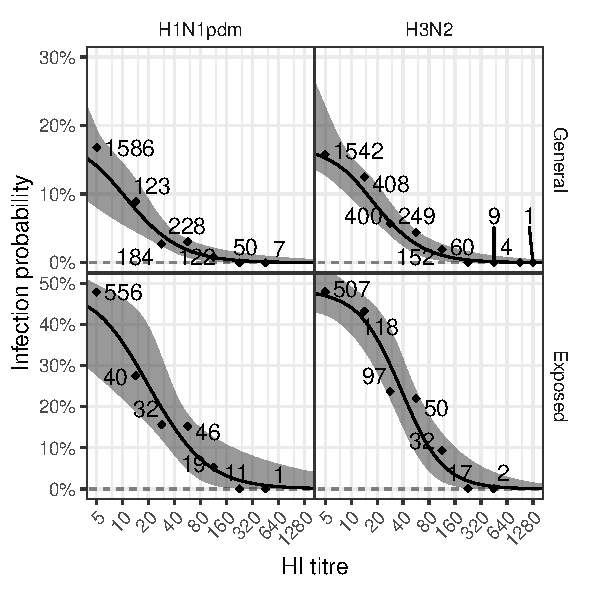
\includegraphics[width=0.8\textwidth]{../fit-sclr-bayesian-plot/hanam-hi-inf.pdf}
	\caption{
	Fitted infection curve and credible interval from the scaled logit model Bayesian fit to Ha Nam data (also shown in Figure \ref{HanamCounts}). The solid line is the median of the posterior distribution. The shaded region is the 95\% credible interval. The dashed line is the prior distribution, i.e. the bounds of the shaded region that would have been obtained if the data contained no information to estimate model parameters. The upper bound is above 90\% and therefore not visible. The points are the infected proportions at the corresponding titre measurements. The numbers next to the points are the total sample size of the corresponding groups. Note that the titre measurements were shifted to midpoints of the corresponding intervals to better represent average underlying titres, e.g. the measurement of 20 was shifted to the log-scale midpoint between 20 and 40 (except the measurement of 5 which represents undetectable titres and the measurement of 1280 which represents titres above the highest detectable level).
	}
	\label{SclrBayesInf}
\end{figure}

\pagebreak

\begin{figure}[htp]
	\centering
	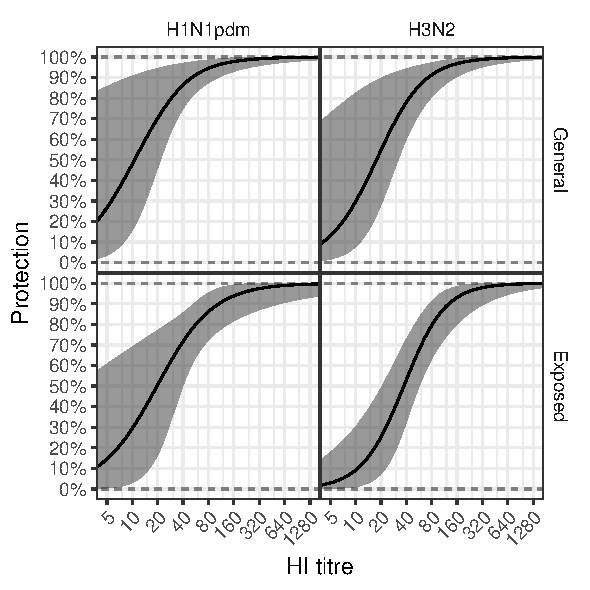
\includegraphics[width=0.8\textwidth]{../fit-sclr-bayesian-plot/hanam-hi-prot.pdf}
	\caption{
	Fitted protection curve and credible interval from the scaled logit model Bayesian fit to Ha Nam data (also shown in Figure \ref{HanamCounts}). The solid line is the median of the posterior distribution. The shaded region is the 95\% credible interval. The dashed line is the prior distribution, i.e. the bounds of the shaded region that would have been obtained if the data contained no information to estimate model parameters.
	}
	\label{SclrBayesProt}
\end{figure}

Limiting the sample to just those exposed to the virus (at least one household infection in a season) improved the precision of the estimates. Despite a fairly large sample, reasonably precise estimates of 50\% protection can only be obtained for the H3N2 virus (inferring from the model fitted to the exposed subset). The general lack of precision in the estimates is likely due to the number of parameters in the model (3 parameters with 1 covariate) and the censored nature of HI titre measurements, particularly the fact that any titre below 10 is undetectable which means that it is impossible to distinguish between many of the observations (e.g. some subjects with undetectable titres may have had a true titre of 9 while others --- of 2, but both were recorded as 5) which makes it harder to estimate the baseline probability (as seen in the credible bounds increasing at small (<10) titres).

%==============================================================================
\section{Kiddyvax application}

The data for this study includes post-vaccination HI titres of subjects who were followed for up to one year for flu infection. The infection status was determined by PCR which was done for everyone who experienced symptoms. This data is shown in Figure \ref{fig:kiddyvax-main-titre}.

\begin{figure}[htp]
	\centering
	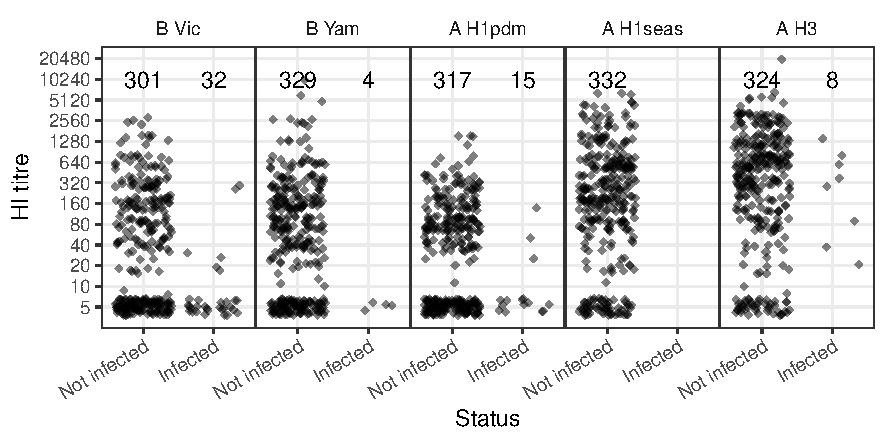
\includegraphics[width=1\textwidth]{../data-plot/kiddyvax-main-titre.pdf}
	\caption{
	Kiddyvax study data. Post-vaccination titres are shown for those who got infected (PCR-confirmed symptomatic infection) over the course of the study and those who did not. Panels correspond to the five tested viruses.
	}
	\label{fig:kiddyvax-main-titre}
\end{figure}

Analyses were done on the data for B Vic and A(H1pdm) viruses in the same way as for the Ha Nam data with the addition of the Cox proportional hazards model.

%\pagebreak
%
\subsection{Scaled logit fit}

The same scaled logit model was fit in the same way using the same prior distributions as for the Ha Nam data. The protection curves are in Figure \ref{fig:kiddyvaxmain-prot-bayes-sclr}. The credible intervals are very broad due to the fact there are very few infections the sample.

\begin{figure}[htp]
	\centering
	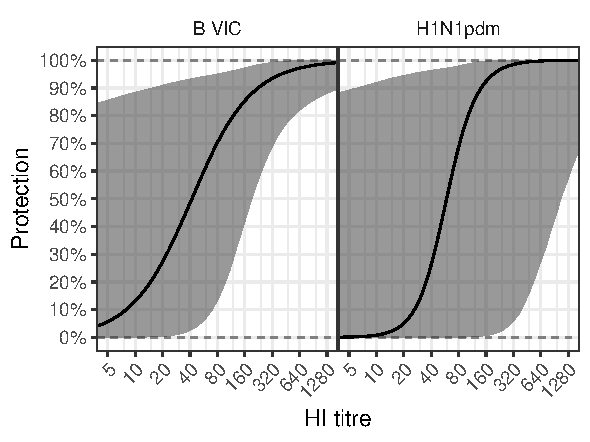
\includegraphics[width=0.8\textwidth]{../fit-sclr-bayesian-plot/kiddyvaxmain-prot.pdf}
	\caption{
Fitted infection curve and credible interval from the scaled logit model Bayesian fit to subsets of kiddyvax data (shown in Figure \ref{fig:kiddyvax-main-titre}). The solid line is the median of the posterior distribution. The shaded region is the 95\% credible interval. The dashed line is the prior distribution, i.e. the bounds of the shaded region that would have been obtained if the data contained no information to estimate model parameters.
	}
	\label{fig:kiddyvaxmain-prot-bayes-sclr}
\end{figure}

\end{document}
